\documentclass[11pt]{article}

\usepackage[margin=2.2cm]{geometry}
\usepackage{xcolor}
\usepackage{forest}
\usepackage{tikz}
\usetikzlibrary{arrows.meta,positioning,decorations.pathreplacing,calc}
\usepackage{amsmath,amssymb,mathtools}
\usepackage{booktabs}
\usepackage{array}
\usepackage{enumitem}
\usepackage{titlesec}
\usepackage{float}
\usepackage[colorlinks=true,linkcolor=teal!70!black,citecolor=teal,urlcolor=teal]{hyperref}
\usepackage{parskip}
\usepackage{cleveref}

\setlength{\parskip}{0.5\baselineskip}
\titlespacing*{\section}{0pt}{1.5em}{0.6em}
\titlespacing*{\subsection}{0pt}{1.2em}{0.4em}

% ---- automatic "Part N --- Title" section numbering, so \section + \label
% gives both the on-page heading and a working \ref/\cref everywhere else ----
\renewcommand{\thesection}{Part \arabic{section}}
\titleformat{\section}{\normalfont\Large\bfseries}{\thesection}{0.6em}{---\ }

% ---- colors reused across every figure, so the same idea always wears the same color ----
\definecolor{lossless}{HTML}{1f7a6c}   % teal family
\definecolor{lossy}{HTML}{c2622d}      % orange family
\definecolor{prefixcol}{HTML}{6a4c93}  % violet
\definecolor{nonprefixcol}{HTML}{1f6fb2}% blue
\definecolor{dictcol}{HTML}{8a5a2b}    % brown
\definecolor{bestcol}{HTML}{2e8b3d}    % green, "best in class" marker
\definecolor{warncol}{HTML}{b3261e}    % red, "error / impossible" marker
\definecolor{transformcol}{HTML}{2f7d8f}% steel teal, transform-based family
\definecolor{contextcol}{HTML}{a13d63} % magenta, context-modeling family
\definecolor{mmcol}{HTML}{4f6d2f}      % olive, lossless multimedia family

\newcommand{\figdrawnote}[1]{\par\noindent\textbf{\textcolor{gray!60!black}{[Draw on the board here:}} \textit{#1}\textbf{\textcolor{gray!60!black}{]}}\par}

% ---- a colored callout box for direct-to-camera, pause-and-think moments ----
\newcommand{\engage}[3]{%
\begin{center}
\begin{tikzpicture}
\node[draw=#1, thick, rounded corners, fill=#1!6, align=left,
      font=\sffamily\small, text width=0.92\linewidth, inner sep=9pt]
      {\textbf{\textcolor{#1}{#2}}\; #3};
\end{tikzpicture}
\end{center}
}

\title{\Large\bfseries Data Compression Overview\\[4pt]
\large\normalfont Video script with synchronized blackboard figures}
\author{}
\date{}

\begin{document}
\maketitle
\vspace{-2em}

\noindent This is the lecture notes for the YouTube video, with every figure placed exactly
where it should be drawn. Figures that build up over the course of the video
(the master tree, the Shannon-limit wall) appear more than once, each time
showing only what should be on the board \emph{at that point} -- draw onto the
same space rather than starting over.

\section{Lossless vs. lossy}
\label{sec:lossless-lossy}

This video gives you a bird's-eye view of data compression algorithms and techniques. We won't go deep into any single algorithm here. 
However, this high-level view is critical to understanding the overall field of data compression. More importantly, it helps you see where the algorithms in this beautiful YouTube course fit within the bigger picture.
 During the video, you'll be creating a large tree diagram. This shows the hierarchy of compression algorithms
 and techniques. A leaf of the tree will have an actual algorithm, whereas a non-leaf will have the categories that algorithms belong to. Let's start!

Every data compression algorithm falls into one of two broad categories: lossless and lossy.

\begin{figure}[H]
\centering
\begin{forest}
for tree={
  draw, rounded corners, align=center, l sep+=12pt, s sep+=14pt,
  edge={-{Latex[length=2mm]}}, anchor=north, child anchor=north,
  font=\sffamily\small, inner sep=5pt
}
[Data compression, fill=gray!10, draw=gray!70
  [Lossless, fill=lossless!12, draw=lossless]
  [Lossy, fill=lossy!12, draw=lossy]
]
\end{forest}
\caption{The master tree, stage 1. Just the root and the
two top-level branches -- this same tree keeps growing for the rest of the
video.}
\label{fig:master-tree-stage1}
\end{figure}

Let's understand exactly what separates these two categories. For that,
let's look at a simple block diagram.

Imagine you have some original data. We'll call it $x$. This data goes into
a compressor, also called an encoder. What comes out the other side is a
smaller, compressed version of that data. We'll call it $c$. Later, when you
want your data back, you take that compressed data $c$ and feed it into a
decompressor, also called a decoder. What comes out is the recovered data.
We'll call it $\bar{x}$.

\begin{figure}[H]
\centering
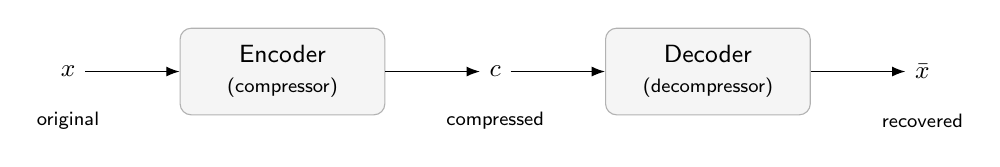
\begin{tikzpicture}[
  box/.style={draw, rounded corners, align=center, font=\sffamily\small, inner sep=6pt, minimum height=1.1cm, minimum width=2.6cm},
  lbl/.style={font=\sffamily\small},
  >=Latex
]
\node[lbl] (x) {$x$};
\node[box, right=12mm of x, fill=gray!8, draw=gray!60] (enc) {Encoder\\{\scriptsize (compressor)}};
\node[lbl, right=12mm of enc] (c) {$c$};
\node[box, right=12mm of c, fill=gray!8, draw=gray!60] (dec) {Decoder\\{\scriptsize (decompressor)}};
\node[lbl, right=12mm of dec] (xbar) {$\bar{x}$};

\draw[->] (x) -- (enc);
\draw[->] (enc) -- (c);
\draw[->] (c) -- (dec);
\draw[->] (dec) -- (xbar);

\node[font=\sffamily\scriptsize, below=2mm of x] {original};
\node[font=\sffamily\scriptsize, below=2mm of c] {compressed};
\node[font=\sffamily\scriptsize, below=2mm of xbar] {recovered};
\end{tikzpicture}
\caption{The encoder/decoder pipeline. Every other figure
in this video about lossless vs.\ lossy is really just zooming in on what
happens to $\bar{x}$ at the very end of this diagram.}
\label{fig:pipeline}
\end{figure}

The entire difference between lossless and lossy compression comes down to
one question. How does $\bar{x}$ compare to the original $x$. In lossless
compression, $\bar{x}$ is always identical to $x$. No matter what the input
was, you are guaranteed to get back the exact original data, bit for bit. In
lossy compression, $\bar{x}$ is not identical to $x$. Some information was
discarded during the encoding process. That information is gone for good. So
what you get back is only an approximation of the original. It is not an
exact copy.

\begin{figure}[H]
\centering
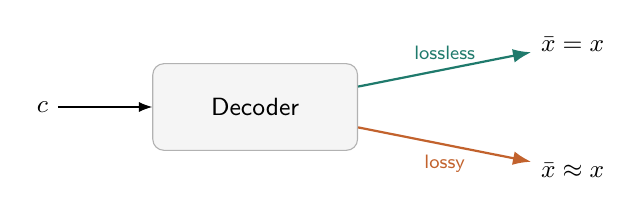
\begin{tikzpicture}[
  box/.style={draw, rounded corners, align=center, font=\sffamily\small, inner sep=6pt, minimum height=1.1cm, minimum width=2.6cm},
  lbl/.style={font=\sffamily\small},
  >=Latex
]
\node[box, fill=gray!8, draw=gray!60] (dec) {Decoder};
\node[lbl, left=12mm of dec] (c) {$c$};
\draw[->] (c) -- (dec);

\node[lbl, right=22mm of dec, yshift=8mm] (los) {$\bar{x} = x$};
\node[lbl, right=22mm of dec, yshift=-8mm] (lossy) {$\bar{x} \approx x$};

\draw[->, lossless, thick] (dec) -- (los) node[midway, above, font=\sffamily\scriptsize, lossless] {lossless};
\draw[->, lossy, thick] (dec) -- (lossy) node[midway, below, font=\sffamily\scriptsize, lossy] {lossy};
\end{tikzpicture}
\caption{The fork that defines the whole field: exact
recovery (teal, lossless) or approximate recovery (orange, lossy). This
annotation sits directly on top of \cref{fig:pipeline}'s decoder output.}
\label{fig:fork}
\end{figure}

It makes sense to use lossy compression when the data is multimedia. That
means audio, video, or images. Losing some data in exchange for better
compression might not even be visible to the naked eye. It might not even be
audible to human ears. But in every other case, you need the data to come
back exactly as it was. Think of the textual records of government
employees. In those cases, you resort to lossless compression instead.

\section{The Shannon limit}
\label{sec:shannon-limit}

Before we divide lossless compression into its different categories, let's
first discuss one fundamental idea. It is one of the greatest theoretical
results in data compression. It is called the Shannon limit.

Claude Shannon showed that every source of data has a compression limit.
This result is known as Shannon's source coding theorem. It tells you the
maximum amount by which the data can be compressed without losing any
information. The limit depends on the amount of information, or
uncertainty, in the source. This quantity is called entropy.

\begin{figure}[H]
\centering
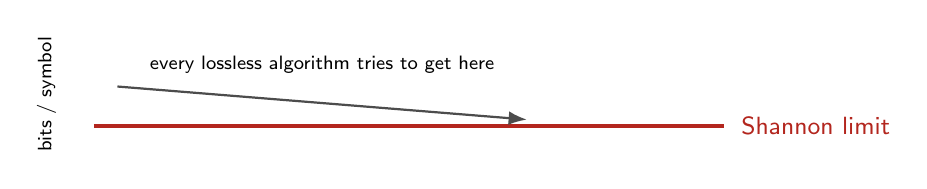
\begin{tikzpicture}[
  >=Latex, font=\sffamily\small
]
\draw[warncol, very thick] (0,0) -- (8,0);
\node[warncol, right] at (8.1,0) {Shannon limit};
\draw[->, gray!60!black, thick] (0.3,0.5) -- (5.5,0.08);
\node[font=\sffamily\scriptsize, above] at (2.9,0.55) {every lossless algorithm tries to get here};
\node[font=\sffamily\scriptsize, rotate=90] at (-0.6,0.4) {bits / symbol};
\end{tikzpicture}
\caption{The Shannon limit, stage 1: a wall that no
lossless algorithm can cross, with one generic arrow approaching it. No
specific algorithms yet -- those get added to this same wall much later, in
\cref{fig:shannon-limit-full}.}
\label{fig:shannon-limit-stage1}
\end{figure}

I have separate videos on entropy and the Shannon limit, so I won't discuss
them in detail here. The key idea is simple. No lossless compression
algorithm, no matter how clever, can achieve an average compressed size
below this limit.

So although the algorithms we are about to study are very different, they
all have the same goal. They try to compress data as close to the Shannon
limit as possible while remaining fast and memory efficient.

\section{The five families of lossless compression}
\label{sec:five-families}

With that in mind, lossless compression can be divided into five categories.
Number one, entropy coding. Number two, dictionary or LZ family. Number
three, transform-based compression. Number four, context modeling. And
number five, multimedia, formats that combine the first four families,
specialized for video, images, and audio.

Let us first briefly describe each of these categories. Then we will zoom
into each one and build more tree diagrams.

\begin{figure}[H]
\centering
\begin{forest}
for tree={
  draw, rounded corners, align=center, l sep+=12pt, s sep+=10pt,
  edge={-{Latex[length=2mm]}}, anchor=north, child anchor=north,
  font=\sffamily\small, inner sep=5pt
}
[Data compression, fill=gray!10, draw=gray!70
  [Lossless, fill=lossless!12, draw=lossless
    [Entropy\\coding, fill=lossless!6, draw=lossless!70]
    [Dictionary\\/ LZ, fill=lossless!6, draw=lossless!70]
    [Transform\\based, fill=lossless!6, draw=lossless!70]
    [Context\\modeling, fill=lossless!6, draw=lossless!70]
    [Multimedia, fill=lossless!6, draw=lossless!70]
  ]
  [Lossy, fill=lossy!12, draw=lossy]
]
\end{forest}
\caption{The master tree, stage 2: Lossless gains its
five children. The first four are algorithmic families; the fifth,
multimedia, is built by combining them, specialized for video, images, and
audio -- we'll see exactly how in \ref{sec:multimedia}. Lossy is still left empty on
purpose -- it is not covered in this video.}
\label{fig:master-tree-stage2}
\end{figure}

Let's start with entropy coding. Entropy coding is a family of techniques.
These techniques assign shorter codes to more probable symbols. They assign
longer codes to less probable ones. For example, in English text, the letter
$e$ appears much more often than the letter $x$. So an entropy coder would
assign a shorter code to $e$. It would assign a longer code to $x$.

\begin{figure}[H]
\centering
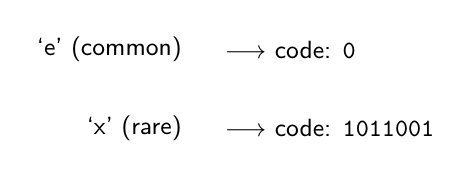
\begin{tikzpicture}[font=\sffamily\small]
\node[anchor=east] at (0,0.5) {`e' (common)};
\node[anchor=west] at (0.3,0.5) {$\longrightarrow$ code: \texttt{0}};
\node[anchor=east] at (0,-0.5) {`x' (rare)};
\node[anchor=west] at (0.3,-0.5) {$\longrightarrow$ code: \texttt{1011001}};
\end{tikzpicture}
\caption{The intuition behind every entropy coder, before
any formal definitions: common symbols get short codes, rare symbols get
long ones.}
\label{fig:entropy-intuition}
\end{figure}

This idea is actually quite intuitive. Symbols that occur more frequently
should take fewer bits to represent. Symbols that occur less frequently can
afford to use more bits. As a result, the average number of bits per symbol
goes down. This is how entropy coding approaches the Shannon limit we just
talked about.

\section{Entropy coding: prefix vs. non-prefix}
\label{sec:entropy-coding}

If we zoom into entropy coding, we find two further groups of algorithms.
These are prefix coding and non-prefix coding.

\begin{figure}[H]
\centering
\begin{forest}
for tree={
  draw, rounded corners, align=center, l sep+=12pt, s sep+=10pt,
  edge={-{Latex[length=2mm]}}, anchor=north, child anchor=north,
  font=\sffamily\small, inner sep=5pt
}
[Entropy coding, fill=lossless!10, draw=lossless!70
  [Prefix coding\\{\scriptsize whole-bit codewords}, fill=prefixcol!10, draw=prefixcol]
  [Non-prefix coding\\{\scriptsize fractional-bit codewords}, fill=nonprefixcol!10, draw=nonprefixcol]
]
\end{forest}
\caption{The master tree, stage 3: Entropy Coding gains
its two children. Violet = prefix coding, blue = non-prefix coding -- these
two colors are reused for the rest of the entropy-coding section.}
\label{fig:entropy-children}
\end{figure}

A prefix code is a type of code where no codeword is the prefix of any other
codeword. This means you can read a stream of bits from left to right. And
you can always tell exactly where one codeword ends. There is no ambiguity.

For example, consider this mapping. $A$ is encoded as \texttt{0}. $B$ is
encoded as \texttt{10}. $C$ is encoded as \texttt{110}. $D$ is encoded as
\texttt{111}. This is a prefix code. None of these codewords starts with
another complete codeword.

\begin{figure}[H]
\centering
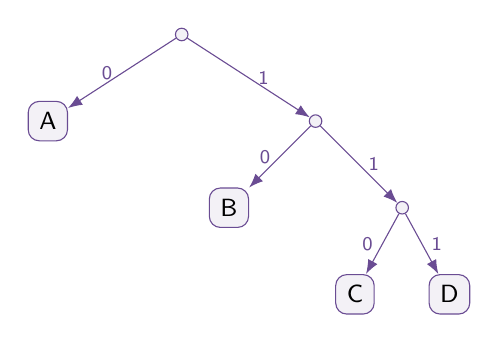
\begin{tikzpicture}[
  level distance=11mm,
  every node/.style={font=\sffamily\small},
  edge from parent/.style={draw, -{Latex[length=1.8mm]}, prefixcol},
  level 1/.style={sibling distance=34mm},
  level 2/.style={sibling distance=22mm},
  level 3/.style={sibling distance=12mm},
  leaf/.style={draw, rounded corners, fill=prefixcol!8, draw=prefixcol, inner sep=4pt},
  internal/.style={circle, draw=prefixcol, fill=prefixcol!8, inner sep=1.6pt}
]
\node[internal] (root) {}
  child { node[leaf] {A} edge from parent node[left, font=\sffamily\scriptsize] {0} }
  child { node[internal] (n1) {}
    child { node[leaf] {B} edge from parent node[left, font=\sffamily\scriptsize] {0} }
    child { node[internal] (n2) {}
      child { node[leaf] {C} edge from parent node[left, font=\sffamily\scriptsize] {0} }
      child { node[leaf] {D} edge from parent node[right, font=\sffamily\scriptsize] {1} }
      edge from parent node[right, font=\sffamily\scriptsize] {1}
    }
    edge from parent node[right, font=\sffamily\scriptsize] {1}
  };
\end{tikzpicture}
\caption{A valid prefix code as a binary tree: $A=0$,
$B=10$, $C=110$, $D=111$. Every letter is a \emph{leaf} -- none of them sits
on the path to another letter, which is exactly what ``prefix-free'' means.}
\label{fig:prefix-tree}
\end{figure}

Now consider this mapping instead. $A$ is encoded as \texttt{0}. $B$ is
encoded as \texttt{01}. $C$ is encoded as \texttt{10}. $D$ is encoded as
\texttt{11}. This is not a prefix code. The codeword for $A$, which is
\texttt{0}, is a prefix of the codeword for $B$, which is \texttt{01}. This
creates ambiguity when decoding.

\begin{figure}[H]
\centering
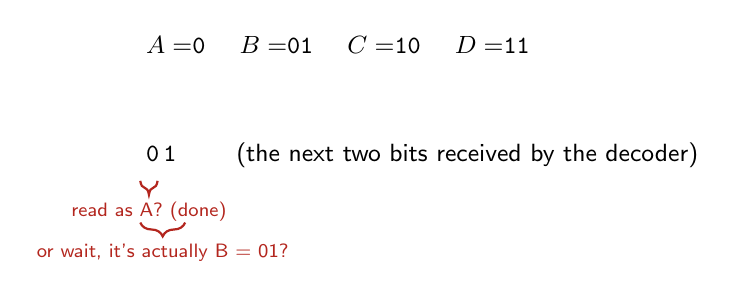
\begin{tikzpicture}[font=\sffamily\small]
\node[anchor=west] (mapping) at (0,1.4) {$A=$\texttt{0} \quad $B=$\texttt{01} \quad $C=$\texttt{10} \quad $D=$\texttt{11}};

\node[anchor=west] (bits) at (0,0) {\texttt{0}\,\texttt{1} \quad\quad (the next two bits received by the decoder)};

\draw[warncol, thick, decorate, decoration={brace, amplitude=5pt, mirror}] (0.05,-0.32) -- (0.27,-0.32) node[midway, below=4pt, warncol, font=\sffamily\scriptsize] {read as A? (done)};
\draw[warncol, thick, decorate, decoration={brace, amplitude=5pt, mirror}] (0.05,-0.85) -- (0.62,-0.85) node[midway, below=4pt, warncol, font=\sffamily\scriptsize] {or wait, it's actually B = 01?};
\end{tikzpicture}
\caption{Why this mapping is ambiguous: after seeing the
single bit \texttt{0}, the decoder cannot tell whether to stop (it's $A$) or
keep reading (it might be the start of $B=01$). This is the one ``error''
figure in the section, marked in red.}
\label{fig:ambiguous-code}
\end{figure}

Shannon coding, Shannon-Fano coding, and Huffman coding are all prefix
codes. Shannon coding takes each symbol's ideal code length, $-\log_2 p$,
and rounds it up to the nearest integer to get that symbol's codeword
length. Shannon-Fano works top-down, repeatedly splitting
the sorted symbol list into two balanced halves. Huffman coding builds the
optimal prefix code for a given probability distribution using a greedy
tree-construction algorithm. Huffman is optimal among all prefix codes for a
memoryless source.

There's a fourth prefix code worth naming here: Rice coding. It's still
entropy coding in the same sense as the other three -- common values get
short codewords, rare values get long ones -- but it gets its probabilities
a different way. Huffman, Shannon, and Shannon-Fano all estimate the
probability of every symbol by measuring the data and building an explicit
table. Rice coding instead assumes the data already follows one specific,
very common shape: a geometric distribution, where small values are likely
and large values get exponentially rarer. That shape happens to match
prediction residuals from audio and image compression almost perfectly. To
encode a value, Rice coding splits it into a quotient and a remainder,
writes the quotient in unary, a string of \texttt{1}s ended by a
\texttt{0}, so smaller quotients really do get shorter codewords, and the
remainder in a fixed number of bits set by a single tunable parameter $k$.
Golomb coding, Rice coding's more general parent, is provably the optimal
prefix code for a geometric source; Rice coding is just the special,
division-free case where that parameter is a power of two. That's the real
difference from the rest of this section: not that it ignores probability,
but that it gets probability from a formula instead of a frequency count,
which is exactly why it's cheap enough to refit block by block rather than
requiring a full pass over the data up front the way Huffman does. We'll
see it again with FLAC in \ref{sec:multimedia}.

Prefix codes are constrained by the Kraft McMillan inequality. One important
consequence of this constraint is that every codeword must have an integer
number of bits. In our earlier example, $A$ was assigned a code of length 1.
$B$ was assigned a code of length 2. $C$ and $D$ were both assigned codes of
length 3. These lengths are all integers. We cannot assign $D$ a code of
length 2.4 in Huffman coding.

Because of this restriction, Huffman coding cannot always match the exact
entropy of the source. So it cannot always reach the Shannon limit.
Arithmetic coding is different. It is a non-prefix entropy coding method. It
can assign each symbol a code of fractional length. So in our example, a
symbol like $D$ could actually be assigned a code of length 2.4.

\begin{figure}[H]
\centering
\begin{tabular}{@{}lcccc@{}}
\toprule
\textbf{Symbol} & \textbf{Probability} & \textbf{Huffman (prefix)} & \textbf{Arithmetic (non-prefix)} \\
\midrule
$A$ & 0.43 & 1 bit & 1.1 bits \\
$B$ & 0.25 & 2 bits & 1.9 bits \\
$C$ & 0.14 & 3 bits & 2.7 bits \\
$D$ & 0.18 & 3 bits & \textcolor{warncol}{\textbf{2.4 bits}} \\
\midrule
\multicolumn{2}{@{}l}{\textbf{Average length (bits/symbol)}} & 1.89 bits & \textcolor{bestcol}{\textbf{1.76 bits}} \\
\bottomrule
\end{tabular}
\caption{Why Huffman can't always reach the entropy
limit: every Huffman codeword length is a whole number (violet column), while
a non-prefix coder like Arithmetic coding can use fractional lengths (blue
column) -- a length of 2.4 bits, marked in red, is simply impossible for $D$
under Huffman coding. The probability column (derived from each symbol's
ideal code length, $p \approx 2^{-\text{length}}$) lets us actually weigh
these lengths: averaged over how often each symbol occurs, Huffman lands at
1.89 bits/symbol, while Arithmetic coding lands at 1.76 bits/symbol (green)
-- a real, measurable gap, not just a per-symbol curiosity.}
\label{fig:huffman-vs-arithmetic}
\end{figure}

Because of this, arithmetic coding can often get very close to the Shannon
limit. In many cases it gets closer than Huffman coding does. This means it
can offer a noticeably better compression ratio. But arithmetic coding is
also noticeably slower. It relies on fractional arithmetic, including
division. To solve this problem, researchers developed range coding. Range
coding uses only integer arithmetic. It avoids division entirely. Range
coding gives you exactly the same compression ratio as arithmetic coding.
But it runs faster.

More recently, many streaming applications have started using entropy
coding. One example is Zstandard, which is used by companies like Netflix and
YouTube. For these applications, even range coding is not fast enough. Users
could experience an annoying delay during streaming. To solve this,
researchers developed a family of algorithms called ANS. These are faster
than both arithmetic coding and range coding. But that extra speed comes at a
small cost. ANS gives you a slightly lower compression ratio in exchange,
very close to arithmetic and range coding but not quite as good. Within this
family, rANS, which stands for range ANS, is best suited for parallel
computing. Most streaming compression tools instead use tANS, which stands
for table ANS. tANS is the fastest of them all, since both encoding and
decoding reduce to simple table lookups.

\begin{figure}[H]
\centering
\resizebox{\textwidth}{!}{%
\begin{forest}
for tree={
  draw, rounded corners, align=center, l sep+=12pt, s sep+=8pt,
  edge={-{Latex[length=2mm]}}, anchor=north, child anchor=north,
  font=\sffamily\small, inner sep=5pt
}
[Entropy coding, fill=lossless!10, draw=lossless!70
  [Prefix coding, fill=prefixcol!10, draw=prefixcol
    [Huffman\\{\scriptsize optimal general prefix}, fill=prefixcol!6, draw=prefixcol]
    [Rice\\{\scriptsize optimal geometric, fastest prefix}, fill=prefixcol!6, draw=prefixcol]
    [Shannon\\{\scriptsize suboptimal prefix}, fill=prefixcol!6, draw=prefixcol]
    [Shannon-Fano\\{\scriptsize suboptimal prefix}, fill=prefixcol!6, draw=prefixcol]
  ]
  [Non-prefix coding, fill=nonprefixcol!10, draw=nonprefixcol
    [Arithmetic\\{\scriptsize best ratio, slowest}, fill=nonprefixcol!6, draw=nonprefixcol]
    [Range coding\\{\scriptsize best ratio, faster}, fill=nonprefixcol!6, draw=nonprefixcol]
    [rANS\\{\scriptsize near-best, fast, parallel}, fill=nonprefixcol!6, draw=nonprefixcol]
    [tANS\\{\scriptsize near-best, fastest}, fill=bestcol!12, draw=bestcol]
  ]
]
\end{forest}%
}
\caption{The entropy-coding branch, fully grown. Green
marks tANS as the fastest of the eight -- pure table lookups, no arithmetic at
all.}
\label{fig:entropy-full}
\end{figure}

So here is how these seven entropy coders actually compare. Huffman is the
quickest and simplest to build, but it gives up the most compression ratio,
since it's stuck with whole numbers of bits. Shannon and Shannon-Fano are
also prefix codes, but neither is guaranteed optimal even among prefix codes
-- Huffman always does at least as well. Arithmetic coding and range coding
sit at the other end. They give you the best possible compression ratio,
right up against the Shannon limit. Between the two, range coding is faster
than arithmetic coding, since it avoids division. rANS and tANS sit in
between on ratio, very close to arithmetic and range coding but not quite as
good, and they are the fastest of the group when it comes to actually running
the encoder and decoder, with tANS being the fastest of all since it relies
purely on table lookups.

Let's pin the comparison down exactly, with two ranked tables.

\begin{figure}[H]
\centering
\begin{tabular}{@{}cp{4.0cm}p{6.5cm}@{}}
\toprule
\textbf{Rank} & \textbf{Algorithm(s)} & \textbf{Why} \\
\midrule
1 & \textcolor{nonprefixcol}{Arithmetic}, \textcolor{nonprefixcol}{Range} &
Tied. Both use fractional-length codewords and get essentially as close to
the Shannon limit as possible. Range coding is just an integer
reformulation of arithmetic coding -- same ratio. \\[4pt]
2 & \textcolor{nonprefixcol}{rANS}, \textcolor{bestcol}{tANS} &
Tied. Also non-prefix, fractional-effective-length coders, so they get very
close to Arithmetic/Range -- but the table-driven, finite-precision approach
gives up a small, deliberate amount of ratio in exchange for speed. \\[4pt]
3 & \textcolor{prefixcol}{Huffman} &
Optimal \emph{among prefix codes} for any distribution. Locked into
whole-bit codewords, so it can't match the non-prefix coders above it, but
better than any other prefix coder in general. \\[4pt]
4 & \textcolor{prefixcol}{Rice} &
Optimal \emph{among prefix codes} specifically for geometric distributions.
On geometric data, matches Huffman's ratio; on non-geometric data, performs
worse. Its advantage is speed and simplicity, not ratio. \\[4pt]
5 & \textcolor{prefixcol}{Shannon}, \textcolor{prefixcol}{Shannon-Fano} &
Tied. Both are prefix codes like Huffman, but neither is guaranteed optimal
even among prefix codes -- Huffman always does at least as well as either of
them. \\
\bottomrule
\end{tabular}
\caption{All entropy coders we've named, ranked by
compression ratio, best to worst. Colors match the prefix/non-prefix split
from \cref{fig:entropy-children,fig:entropy-full}.}
\label{fig:entropy-ratio-rank}
\end{figure}

Now let's rank the same seven algorithms a completely different way: by speed.

\begin{figure}[H]
\centering
\begin{tabular}{@{}cp{4.2cm}p{6.8cm}@{}}
\toprule
\textbf{Rank} & \textbf{Algorithm(s)} & \textbf{Why} \\
\midrule
1 & \textcolor{bestcol}{tANS} &
Fastest of all. Encoding and decoding reduce to pure table lookups -- no
arithmetic operations at all. \\[4pt]
2 & \textcolor{prefixcol}{Rice} &
Extremely fast. No probability table needs to be built -- the distribution
is assumed from a single parameter $k$, so encoding/decoding is just simple
bit manipulation: unary for the quotient, fixed bits for the remainder. \\[4pt]
3 & \textcolor{prefixcol}{Huffman}, \textcolor{prefixcol}{Shannon},
\textcolor{prefixcol}{Shannon-Fano} &
Tied. All three are prefix codes -- encode/decode is a simple lookup of a
fixed bit pattern per symbol, structurally similar and similarly fast
regardless of which one assigns the codewords. (Building the table is
another matter -- Huffman's table construction is fast, Shannon/Shannon-Fano
are faster to build but worse on ratio.) \\[4pt]
4 & \textcolor{nonprefixcol}{rANS} &
Fast, but each symbol still requires a bit of integer arithmetic to update
the state, so it's a step behind the pure-lookup tANS. \\[4pt]
5 & \textcolor{nonprefixcol}{Range} &
Uses integer arithmetic with renormalization but avoids division -- faster
than arithmetic coding, slower than the table-driven methods above. \\[4pt]
6 & \textcolor{nonprefixcol}{Arithmetic} &
Slowest. Needs high-precision, renormalizing fractional arithmetic,
historically including division per symbol. \\
\bottomrule
\end{tabular}
\caption{The same entropy coders, ranked by
compression speed, fastest to slowest. Notice the ranking barely resembles
\cref{fig:entropy-ratio-rank}'s ranking -- the fastest coder (tANS) is tied
for second-worst on ratio, Rice is tied for second-fastest but ranks below
Huffman on general ratio, and the three slowest-to-rank-1 coders on ratio
(Huffman, Shannon, Shannon-Fano) are tied for third-fastest here.}
\label{fig:entropy-speed-rank}
\end{figure}

\engage{prefixcol}{Side note:}{Huffman's reputation for being ``fast''
usually refers to how quickly its code \emph{table} can be built -- it's a
simple, greedy tree construction. That's a separate claim from how fast
encoding and decoding run per symbol once the table already exists, which is
exactly why those two ideas land in different tables above rather than
getting conflated into one.}

\begin{figure}[H]
\centering
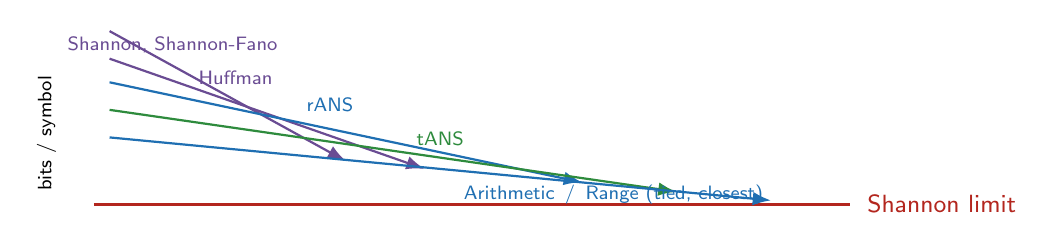
\begin{tikzpicture}[
  >=Latex, font=\sffamily\small
]
\draw[warncol, very thick] (0,0) -- (9.6,0);
\node[warncol, right] at (9.7,0) {Shannon limit};
\node[font=\sffamily\scriptsize, rotate=90] at (-0.6,0.9) {bits / symbol};

\draw[->, prefixcol, thick] (0.2,2.2) -- (3.2,0.55);
\node[prefixcol, font=\sffamily\scriptsize, above] at (1.0,1.8) {Shannon, Shannon-Fano};

\draw[->, prefixcol, thick] (0.2,1.85) -- (4.2,0.45);
\node[prefixcol, font=\sffamily\scriptsize, above] at (1.8,1.4) {Huffman};

\draw[->, nonprefixcol, thick] (0.2,1.55) -- (6.2,0.28);
\node[nonprefixcol, font=\sffamily\scriptsize, above] at (3.0,1.05) {rANS};

\draw[->, bestcol, thick] (0.2,1.2) -- (7.4,0.16);
\node[bestcol, font=\sffamily\scriptsize, above] at (4.4,0.62) {tANS};

\draw[->, nonprefixcol, thick] (0.2,0.85) -- (8.6,0.05);
\node[nonprefixcol, font=\sffamily\scriptsize, below=1pt] at (6.6,0.40) {Arithmetic \,/\, Range (tied, closest)};
\end{tikzpicture}
\caption{The Shannon limit wall, fully labeled. Arithmetic
and Range coding are tied for closest to the limit -- that is the entire
reason they exist. rANS and tANS trade a small, deliberate gap from the limit
for a large gain in speed. Huffman is further from the wall, since it is
locked into whole-bit codewords. Shannon and Shannon-Fano are furthest, since
they aren't even optimal among prefix codes. Colors match \cref{fig:entropy-full}.}
\label{fig:shannon-limit-full}
\end{figure}

\section{Dictionary compression: the LZ family}
\label{sec:dictionary-lz}

Next, we move to dictionary-based compression algorithms. They mostly
belong to the LZ family. At a high level, we can divide them into LZ77 and
LZ78.

Dictionary compressors like LZ77 replace repeated byte patterns with a short reference pointing back to where that pattern last appeared, 
using a sliding window of recent data to keep the reference small and efficient.

\begin{figure}[H]
\centering
\begin{forest}
for tree={
  draw, rounded corners, align=center, l sep+=12pt, s sep+=10pt,
  edge={-{Latex[length=2mm]}}, anchor=north, child anchor=north,
  font=\sffamily\small, inner sep=5pt
}
[Data compression, fill=gray!10, draw=gray!70
  [Lossless, fill=lossless!12, draw=lossless
    [Entropy\\coding, fill=lossless!6, draw=lossless!70]
    [Dictionary\\/ LZ, fill=dictcol!10, draw=dictcol
      [LZ77\\{\scriptsize sliding window}, fill=dictcol!6, draw=dictcol]
      [LZ78\\{\scriptsize growing dictionary}, fill=dictcol!6, draw=dictcol]
    ]
    [Transform\\based, fill=lossless!6, draw=lossless!70]
    [Context\\modeling, fill=lossless!6, draw=lossless!70]
    [Multimedia, fill=lossless!6, draw=lossless!70]
  ]
  [Lossy, fill=lossy!12, draw=lossy]
]
\end{forest}
\caption{The master tree, stage 4: Dictionary / LZ gains
its two children, LZ77 and LZ78, drawn in a new color (brown) so it's
visually distinct from the entropy-coding branch. Transform based, context
modeling, and multimedia are still waiting their turn, in Parts 6 through 8.}
\label{fig:master-tree-stage4}
\end{figure}

The key difference is this. LZ77 uses a sliding window. This makes it memory
constrained. LZ78 instead uses a growing dictionary.

\begin{figure}[H]
\centering
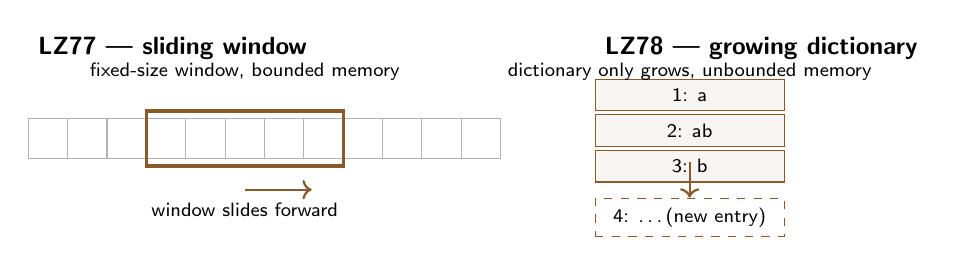
\begin{tikzpicture}[font=\sffamily\small]
% LZ77: sliding window over a fixed-length tape
\node[anchor=west] at (0,3.4) {\textbf{LZ77 --- sliding window}};
\foreach \i in {0,...,11}{
  \draw[gray!60] (\i*0.5,2.0) rectangle (\i*0.5+0.5,2.5);
}
\draw[dictcol, very thick] (1.5,1.9) rectangle (4.0,2.6);
\draw[->, dictcol, thick] (2.75,1.6) -- (3.6,1.6);
\node[font=\sffamily\scriptsize, below] at (2.75,1.55) {window slides forward};
\node[font=\sffamily\scriptsize] at (2.75,3.5) [yshift=-0.4cm] {fixed-size window, bounded memory};

% LZ78: growing dictionary table
\node[anchor=west] at (7.2,3.4) {\textbf{LZ78 --- growing dictionary}};
\foreach \i/\txt in {0/1: a, 1/2: ab, 2/3: b}{
  \node[draw=dictcol, fill=dictcol!6, font=\sffamily\scriptsize, minimum width=2.4cm] at (8.4,2.8-\i*0.45) {\txt};
}
\draw[->, dictcol, thick] (8.4,1.95) -- (8.4,1.5);
\node[draw=dictcol, dashed, font=\sffamily\scriptsize, minimum width=2.4cm] at (8.4,1.25) {4: \ldots (new entry)};
\node[font=\sffamily\scriptsize] at (8.4,3.5) [yshift=-0.4cm] {dictionary only grows, unbounded memory};
\end{tikzpicture}
\caption{The core contrast between the two LZ branches.
LZ77's window (left) stays the same size and slides over the data it has
already seen. LZ78's dictionary (right) starts empty and gains a new entry
every time a new substring is seen.}
\label{fig:lz77-vs-lz78}
\end{figure}

Most of the algorithms we cover in this course are extensions of LZ77.
Now let's see how LZ77 actually works, at a high level. It slides a
fixed-size window over the data, split into two parts: a search buffer
holding what's already been seen, and a look-ahead buffer holding what's
about to be encoded. Whenever the look-ahead buffer's next string already
appears somewhere in the search buffer, LZ77 replaces it with a short
reference: how far back the match starts, and how long it runs. The window
then slides forward to cover that newly encoded data.

We're skipping real details here -- match-finding strategies, encoding
optimizations, overlapping matches -- since they deserve their own video.
For now, the takeaway is simple: LZ77 swaps repeated patterns for short
references, and almost every dictionary compressor in use today is built
directly on this sliding-window idea.

Here's a tiny example, shown in Figure~\ref{fig:lz77-example}. Say the
look-ahead buffer's next characters are \texttt{abc}, and that exact string
already appeared earlier in the search buffer. Instead of writing
\texttt{a}, \texttt{b}, \texttt{c} all over again, LZ77 just points back to
that earlier copy. Because the window is small, a reference back into it
is almost always shorter than the text it replaces.

\begin{figure}[H]
\centering
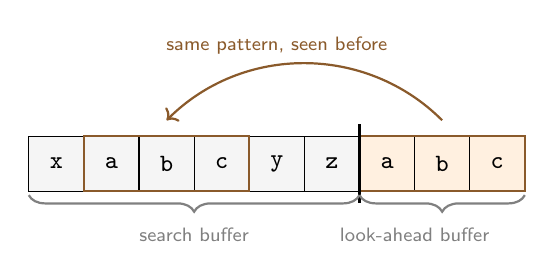
\begin{tikzpicture}[font=\sffamily\small]
% search buffer cells (already seen)
\foreach \i/\c in {0/x,1/a,2/b,3/c,4/y,5/z}{
  \draw[fill=gray!8] (\i*0.7,0) rectangle (\i*0.7+0.7,0.7);
  \node at (\i*0.7+0.35,0.35) {\texttt{\c}};
}
% look-ahead buffer cells (about to be encoded)
\foreach \i/\c in {6/a,7/b,8/c}{
  \draw[fill=orange!12] (\i*0.7,0) rectangle (\i*0.7+0.7,0.7);
  \node at (\i*0.7+0.35,0.35) {\texttt{\c}};
}
% highlight the matching substrings
\draw[thick, dictcol] (1*0.7,0) rectangle (3*0.7+0.7,0.7);
\draw[thick, dictcol] (6*0.7,0) rectangle (8*0.7+0.7,0.7);
% boundary line between the two buffers
\draw[very thick, black] (6*0.7,-0.15) -- (6*0.7,0.85);
% arrow + label
\draw[->, thick, dictcol] (7*0.7+0.35,0.9) to[bend right=45] (2*0.7+0.35,0.9);
\node[dictcol, font=\sffamily\scriptsize] at (4.5*0.7,1.85) {same pattern, seen before};
% buffer braces + labels
\draw[decorate, decoration={brace, amplitude=6pt, mirror}, thick, gray] (0,-0.05) -- (6*0.7,-0.05);
\node[gray, font=\sffamily\scriptsize] at (3*0.7,-0.55) {search buffer};
\draw[decorate, decoration={brace, amplitude=6pt, mirror}, thick, gray] (6*0.7,-0.05) -- (8*0.7+0.7,-0.05);
\node[gray, font=\sffamily\scriptsize] at (7*0.7,-0.55) {look-ahead buffer};
\end{tikzpicture}
\caption*{The second \texttt{abc} doesn't get written out
again -- it's replaced by a reference pointing back to the first one. We'll
unpack exactly what that reference contains in a future video.}
\label{fig:lz77-example}
\end{figure}

Most real-world compressors are exactly this idea, dressed up with a
particular entropy coder on top. DEFLATE is LZ77 combined with Huffman
coding, and it's the engine inside zip, gzip, and PNG -- old, simple, and
everywhere. Zstandard is LZ77 combined with tANS, a much newer design tuned
to get close to DEFLATE's ratio, or better, while running far faster, which
is why companies like Facebook and Netflix use it for everyday compression
at scale. LZMA (Lempel-Ziv-Markov chain algorithm) uses LZ77 with larger
dictionaries and advanced entropy coding (range coding), achieving
excellent compression ratios at the cost of slower speed. Brotli, used in
web compression (HTTP), is a modern LZ77 variant with a static dictionary
of common web strings and Huffman coding, offering better compression than
gzip for text. Snappy, developed by Google, is an extremely fast
LZ77-based compressor with modest compression, optimized for low latency
in databases and real-time systems.

\begin{figure}[H]
\centering
\begin{forest}
for tree={
  draw, rounded corners, align=center, l sep+=10pt, s sep+=8pt,
  edge={-{Latex[length=2mm]}}, anchor=north, child anchor=north,
  font=\sffamily\small, inner sep=4pt
}
[LZ77, fill=dictcol!10, draw=dictcol
  [DEFLATE\\{\scriptsize LZ77 + \textcolor{prefixcol}{Huffman}}, fill=dictcol!6, draw=dictcol]
  [Zstandard\\{\scriptsize LZ77 + \textcolor{bestcol}{tANS}}, fill=dictcol!6, draw=dictcol]
  [LZMA\\{\scriptsize LZ77 + \textcolor{nonprefixcol}{range coding}}, fill=dictcol!6, draw=dictcol]
  [Brotli\\{\scriptsize LZ77 + web dict + \textcolor{prefixcol}{Huffman}}, fill=dictcol!6, draw=dictcol]
  [Snappy\\{\scriptsize LZ77, extremely fast}, fill=dictcol!6, draw=dictcol]
]
\end{forest}
\caption{LZ77 in practice: five real formats, each adding
an entropy coder from \ref{sec:entropy-coding} or a specialized optimization. The ``+Huffman'',
``+tANS'', and ``+range coding'' labels are colored to match
\cref{fig:entropy-full,fig:entropy-ratio-rank,fig:entropy-speed-rank} --
dictionary methods don't replace entropy coding, they hand off to it.}
\label{fig:lz77-formats}
\end{figure}


%%%%
Just like we did with entropy coding, let's compare these five
dictionary-based formats on two dimensions: compression ratio
(Figure~\ref{fig:dict-ratio-rank}) and speed
(Figure~\ref{fig:dict-speed-rank}).

\begin{figure}[H]
\centering
\begin{tabular}{@{}cp{4.0cm}p{6.5cm}@{}}
\toprule
\textbf{Rank} & \textbf{Algorithm} & \textbf{Why} \\
\midrule
1 & \textcolor{dictcol}{LZMA} &
Best compression ratio among dictionary methods. Uses large dictionaries
(up to 4\,GB) and \textcolor{nonprefixcol}{range coding} for entropy,
enabling excellent ratio at the cost of speed. \\[4pt]
2 & \textcolor{dictcol}{Brotli} &
Excellent ratio, especially on text. Uses a large static dictionary of
common web strings plus \textcolor{prefixcol}{Huffman coding}. Often
outperforms DEFLATE on web content by around 20--26\%. \\[4pt]
3 & \textcolor{dictcol}{Zstandard} &
Very good ratio, tunable from near-DEFLATE to near-LZMA levels. Uses LZ77
plus \textcolor{bestcol}{tANS}, and at higher compression levels typically
beats DEFLATE on ratio while still running at comparable or faster speed.
\\[4pt]
4 & \textcolor{dictcol}{DEFLATE} &
Decent, general-purpose ratio. LZ77 plus \textcolor{prefixcol}{Huffman
coding}. The original universal baseline -- simple, well understood, and
everywhere (zip, gzip, PNG) -- though Zstandard now beats it on ratio in
most benchmarks. \\[4pt]
5 & \textcolor{dictcol}{Snappy} &
Modest compression ratio -- deliberately trades ratio for speed. Designed
for databases and real-time systems where latency matters more than
storage. \\
\bottomrule
\end{tabular}
\caption{Dictionary-based formats ranked by compression ratio, best to
worst. LZMA (range coding) and Brotli (Huffman with web dictionary) lead;
Snappy intentionally sacrifices ratio for speed.}
\label{fig:dict-ratio-rank}
\end{figure}

Figure~\ref{fig:dict-ratio-rank} ranked these formats by compression ratio.
Now let's rank the same five formats by speed, in
Figure~\ref{fig:dict-speed-rank}.

\begin{figure}[H]
\centering
\begin{tabular}{@{}cp{4.0cm}p{6.5cm}@{}}
\toprule
\textbf{Rank} & \textbf{Algorithm} & \textbf{Why} \\
\midrule
1 & \textcolor{dictcol}{Snappy} &
Fastest of all. Minimal dictionary lookups, no entropy coding overhead.
Designed specifically for maximum throughput, with compression ratio as a
secondary concern. \\[4pt]
2 & \textcolor{dictcol}{Zstandard} &
Very fast, especially at lower compression levels. \textcolor{bestcol}{tANS}
is extremely efficient, and the implementation is heavily optimized. Often
matches or exceeds Snappy's decompression speed while compressing better.
\\[4pt]
3 & \textcolor{dictcol}{DEFLATE} &
Moderate speed. \textcolor{prefixcol}{Huffman coding} is fast, but LZ77
match-finding can be expensive. Gzip, built on DEFLATE, has long been the
default wherever ``good enough'' speed was all that mattered. \\[4pt]
4 & \textcolor{dictcol}{Brotli} &
Slower than DEFLATE. The larger dictionary and more complex match-finding
cost extra CPU time. Quality over speed, especially for offline compression
of web assets. \\[4pt]
5 & \textcolor{dictcol}{LZMA} &
Slowest of the five. Large dictionaries and complex
\textcolor{nonprefixcol}{range coding} make it CPU-intensive. Designed for
maximum compression, not speed -- often used for software distribution,
where decompression speed matters more than compression speed. \\
\bottomrule
\end{tabular}
\caption{Dictionary-based formats ranked by compression speed, fastest to
slowest. Notice the ranking is almost the reverse of
Figure~\ref{fig:dict-ratio-rank} -- Snappy is fastest but worst on ratio,
LZMA is best on ratio but slowest.}
\label{fig:dict-speed-rank}
\end{figure}

The key insight from Figures~\ref{fig:dict-ratio-rank} and
\ref{fig:dict-speed-rank} is the same trade-off we saw with entropy coding:
\textbf{you can't have both maximum ratio and maximum speed.} Each format
makes a deliberate choice about where to sit on that spectrum:

\begin{itemize}
\item \textbf{Snappy} prioritizes speed above all else.
\item \textbf{Zstandard} offers the best overall balance -- good ratio with
competitive, often class-leading speed.
\item \textbf{DEFLATE} isn't really on this frontier anymore -- Zstandard
beats it on both ratio and speed in most benchmarks. DEFLATE survives
because it's been the universal default since the 1990s (zip, gzip, PNG),
not because of where it sits on this trade-off.
\item \textbf{Brotli} trades some speed for better ratio, especially on
web content.
\item \textbf{LZMA} goes all-in on ratio, accepting much slower compression.
\end{itemize}




\section{Transform-based compression: the Burrows--Wheeler Transform}
\label{sec:transform-bwt}

We've now covered two of our five lossless families: entropy coding and
dictionary compression. Let's move to the third family. Transform-based
compression.

Here's the core idea. Instead of compressing the data directly, first
transform it into a completely different arrangement of the exact same
symbols. An arrangement that happens to be far easier to compress. Then run
a simple compressor on top of that.

The most famous example of this approach is the Burrows-Wheeler Transform,
or BWT. It is the engine inside the popular bzip2 compressor.

\engage{transformcol}{Pause and guess:}{the Burrows-Wheeler Transform, by
itself, does not save a single bit. Not one. So why would anyone bother
using it? Take a guess, then keep watching.}

Here's how it works. Take your string, and add a unique end marker to it,
say a dollar sign. Now generate every rotation of that string. Sort all of
those rotations alphabetically. The BWT output is simply the last column of
that sorted list.

\begin{figure}[H]
\centering
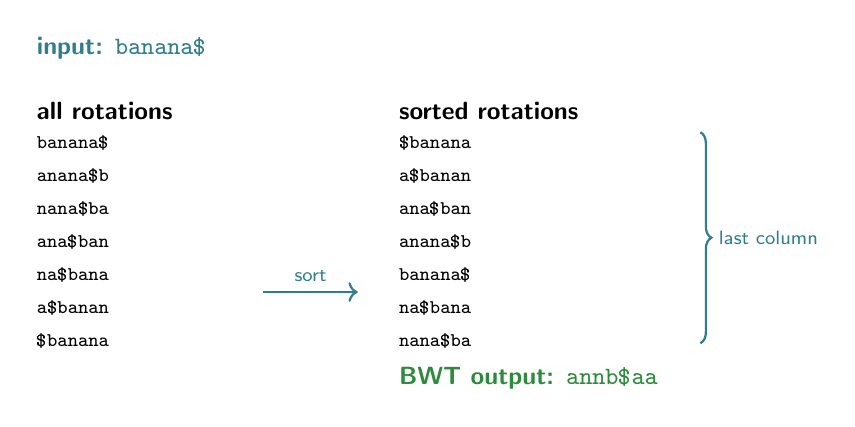
\begin{tikzpicture}[font=\sffamily\small]
\node[anchor=west, transformcol, font=\sffamily\small\bfseries] at (0,5.2) {input: \texttt{banana\$}};

\node[anchor=west] at (0,4.4) {\textbf{all rotations}};
\foreach \i/\txt in {0/banana\$,1/anana\$b,2/nana\$ba,3/ana\$ban,4/na\$bana,5/a\$banan,6/\$banana}{
  \node[font=\sffamily\scriptsize, anchor=west] at (0,4.0-\i*0.42) {\texttt{\txt}};
}

\draw[->, transformcol, thick] (3.0,2.1) -- (4.2,2.1) node[midway, above, font=\sffamily\scriptsize, transformcol] {sort};

\node[anchor=west] at (4.6,4.4) {\textbf{sorted rotations}};
\foreach \i/\txt in {0/\$banana,1/a\$banan,2/ana\$ban,3/anana\$b,4/banana\$,5/na\$bana,6/nana\$ba}{
  \node[font=\sffamily\scriptsize, anchor=west] at (4.6,4.0-\i*0.42) {\texttt{\txt}};
}

\draw[transformcol, thick, decorate, decoration={brace, amplitude=4pt}] (8.55,4.13) -- (8.55,1.45) node[midway, right=3pt, font=\sffamily\scriptsize, transformcol] {last column};

\node[anchor=west, bestcol, font=\sffamily\small\bfseries] at (4.6,1.0) {BWT output: \texttt{annb\$aa}};
\end{tikzpicture}
\caption{The Burrows-Wheeler Transform of \texttt{banana\$},
worked by hand. Every rotation of the input (left) is sorted alphabetically
(right), and the last letter of each sorted row, read top to bottom, is the
BWT output. Notice the output has far more repeated, neighboring letters
than the original string did.}
\label{fig:bwt}
\end{figure}

So why bother? Look closely at the output: \texttt{annb\$aa}. Compare that to
the original: \texttt{banana\$}. The letters haven't changed, and there are
exactly as many of them. But in the BWT output, identical letters are far
more likely to sit right next to each other. That's because sorting groups
together every rotation that shares the same upcoming context. The BWT
itself doesn't compress anything. What it does is rearrange the data so that
a much simpler compressor, typically a move-to-front transform, followed by
run-length encoding, followed by entropy coding, can squeeze it far harder
than it could squeeze the original. That handoff to a simple downstream
compressor is exactly how bzip2 is built.

The ``much simpler compressor'' mentioned above is itself a second
transform: the move-to-front transform, or MTF. By the same definition
used for BWT, MTF qualifies as transform-based compression too -- it
doesn't shrink the data by a single bit on its own, it just rearranges
symbols into a far more compressible shape, then hands off to run-length
and entropy coding to do the actual squeezing.

Here's how it works. Keep a list of every distinct symbol in the data,
in some starting order. For each symbol in the input, output its current
position in that list, then move that symbol to the front of the list.
Symbols that keep repeating, exactly what BWT produces in long runs, end
up at the front of the list almost permanently, so they keep generating
small numbers, often literally zero.

\begin{figure}[H]
\centering
\begin{tabular}{@{}cccc@{}}
\toprule
\textbf{Symbol} & \textbf{List before} & \textbf{Output} & \textbf{List after} \\
\midrule
a & \texttt{\$ a b n} & 1 & \texttt{a \$ b n} \\
n & \texttt{a \$ b n} & 3 & \texttt{n a \$ b} \\
n & \texttt{n a \$ b} & 0 & \texttt{n a \$ b} \\
b & \texttt{n a \$ b} & 3 & \texttt{b n a \$} \\
\$ & \texttt{b n a \$} & 3 & \texttt{\$ b n a} \\
a & \texttt{\$ b n a} & 3 & \texttt{a \$ b n} \\
a & \texttt{a \$ b n} & 0 & \texttt{a \$ b n} \\
\bottomrule
\end{tabular}
\caption{The move-to-front transform applied to the BWT output
\texttt{annb\$aa} from Figure~\ref{fig:bwt}, starting from the alphabet
\texttt{\$ a b n}. Each row outputs the symbol's current position, then
moves that symbol to the front. The MTF output is \texttt{1 3 0 3 3 3 0}
-- mostly small numbers, with three 3's and two 0's, exactly the kind of
skewed, repetitive distribution that run-length and entropy coding
exploit well.}
\label{fig:mtf}
\end{figure}

That output, \texttt{1 3 0 3 3 3 0}, is what bzip2 hands next to
run-length encoding and then entropy coding. None of the three steps,
BWT, MTF, or RLE, compresses anything by itself. Each one just reshapes
the data so the next stage in the pipeline has an easier job.

BWT and MTF aren't the only transforms in this family, either. Delta
encoding replaces each value with its difference from a predicted value,
often just the previous one, turning smoothly changing data into a
stream of small numbers; it's the same idea behind PNG's per-row
prediction filter (\ref{sec:lossy-fill}). The discrete cosine transform and the
discrete wavelet transform, the workhorses behind JPEG and MP3, do the
same job for lossy compression: they convert a signal into frequency
components so that most of the energy lands on a few large coefficients
and everything else can be quantized away almost for free. What unites
all of these, BWT, MTF, delta encoding, DCT, is the same handoff
pattern: rearrange or re-express the data first, then let a simpler
coder do the squeezing.

\begin{figure}[H]
\centering
\begin{forest}
for tree={
  draw, rounded corners, align=center, l sep+=12pt, s sep+=10pt,
  edge={-{Latex[length=2mm]}}, anchor=north, child anchor=north,
  font=\sffamily\small, inner sep=5pt
}
[Transform\\based, fill=transformcol!10, draw=transformcol
  [BWT\\{\scriptsize\parbox{4.4cm}{\centering reorders symbols by context so simple coders can exploit the new runs; powers bzip2}}, fill=transformcol!6, draw=transformcol]
  [MTF\\{\scriptsize\parbox{4.4cm}{\centering turns repeated symbols into small numbers, mostly zeros; usually paired right after BWT}}, fill=transformcol!6, draw=transformcol]
  [Delta /\\DCT\\{\scriptsize\parbox{4.4cm}{\centering predicts each value from its neighbors so only the residual needs coding; used in PNG, JPEG, MP3}}, fill=transformcol!6, draw=transformcol]
]
\end{forest}
\caption{The transform-based branch. None of BWT, MTF, or delta/DCT
compete with entropy coding or LZ -- each is a pre-processing step that
makes whatever comes after it work better.}
\label{fig:transform-branch}
\end{figure}

\section{Context modeling: PPM and context mixing}
\label{sec:context-modeling}

That brings us to the fourth of our five lossless families: context
modeling.

Entropy coding assigns a symbol's code length based on how common that symbol is, overall, across the entire source.
Context modeling asks a sharper question. Forget the overall frequency. How likely is this symbol to appear \emph{right here}, 
given the handful of symbols that just came before it?

Context modeling is effectively an order-\emph{n} entropy model, where $n$ is the size of the context. It estimates the probability of
each symbol conditioned on the $n$ symbols that preceded it, rather than using a single global probability for every symbol.

The flagship algorithm in this family is called PPM, which stands for
Prediction by Partial Matching.

\engage{contextcol}{Quick check:}{if entropy coding already gives common
symbols short codes, what extra trick is context modeling adding on top?
(Answer is in the next paragraph -- try to guess it first.)}

Here is PPM, in plain terms. To predict the next symbol, PPM looks at the
last few symbols it has already seen, that short, recent window is the
\emph{context}, the ``partial match.'' It then checks how often each
possible symbol has followed that exact context before, and turns those
counts into a probability distribution. That distribution gets handed to an
entropy coder, almost always arithmetic coding, which does the actual work
of writing out the bits. And if that exact context has never come up
before, PPM doesn't give up: it escapes down to a shorter context, one
symbol shorter at a time, until it finds one with real statistics behind it.

\begin{figure}[H]
\centering
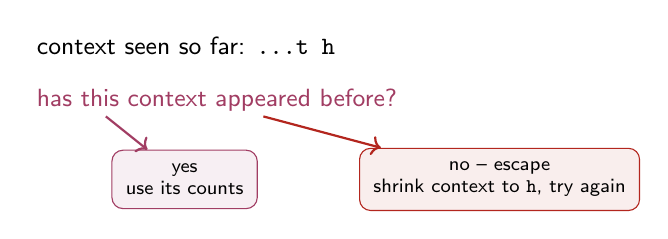
\begin{tikzpicture}[font=\sffamily\small]
\node[anchor=west] at (0,2.6) {context seen so far: \texttt{\ldots t h}};
\node[anchor=west, contextcol] at (0,1.9) {has this context appeared before?};

\node[draw=contextcol, rounded corners, fill=contextcol!8, align=center, font=\sffamily\scriptsize, inner sep=5pt] (yes) at (2.0,0.9) {yes\\use its counts};
\node[draw=warncol, rounded corners, fill=warncol!8, align=center, font=\sffamily\scriptsize, inner sep=5pt] (no) at (6.0,0.9) {no -- escape\\shrink context to \texttt{h}, try again};

\draw[->, contextcol, thick] (1.0,1.7) -- (yes);
\draw[->, warncol, thick] (3.0,1.7) -- (no);
\end{tikzpicture}
\caption{PPM's escape mechanism. If the current context
has statistics, PPM uses them directly (left, teal-magenta). If not, it
shrinks the context by one symbol and tries again (right, red), repeating
until it lands on a context it has actually seen.}
\label{fig:ppm-escape}
\end{figure}

PPM has a more powerful, and much slower, cousin called context mixing, or
CM. Instead of picking one context length and falling back when it fails,
context mixing blends predictions from many different models at once,
different context lengths, even entirely different kinds of models, using a
weighted combination instead of an either-or choice. This family holds the
records for the best compression ratios ever measured, and it's the
approach behind compressors like PAQ and its descendants. The cost is speed:
context mixing can run hundreds of times slower than something like Huffman
coding.

\engage{contextcol}{Fun fact:}{the Hutter Prize is an ongoing competition
that pays out cash for shrinking a fixed 1\,GB sample of Wikipedia text as
small as possible. The idea is that squeezing text harder forces you to
\emph{model} it better, and better modeling of language is a proxy for
general intelligence. Every leading entry for years has been a context
mixing compressor descended from PAQ -- the same family we just met, pushed
to its absolute limit.}

\begin{figure}[H]
\centering
\begin{forest}
for tree={
  draw, rounded corners, align=center, l sep+=12pt, s sep+=10pt,
  edge={-{Latex[length=2mm]}}, anchor=north, child anchor=north,
  font=\sffamily\small, inner sep=5pt
}
[Context\\modeling, fill=contextcol!10, draw=contextcol
  [PPM\\{\scriptsize\parbox{4.4cm}{\centering predicts each symbol from its recent context, escaping to shorter contexts when needed}}, fill=contextcol!6, draw=contextcol]
  [Context\\mixing (CM)\\{\scriptsize\parbox{4.4cm}{\centering blends many context models at once; best ratio of all, but very slow}}, fill=bestcol!12, draw=bestcol]
]
\end{forest}
\caption{The context-modeling branch. Context mixing
(green) sits at the extreme ``best possible ratio'' end of every trade-off
curve we've drawn so far, paid for entirely in speed.}
\label{fig:context-branch}
\end{figure}

\section{The fifth family: multimedia}
\label{sec:multimedia}

We've now met four of the five algorithmic families that make up lossless
compression: entropy coding, dictionary or LZ, transform based, and context
modeling. Time for the fifth one we promised back in \ref{sec:five-families}: multimedia.

Earlier in this video I said multimedia, video, images, and audio, is the
classic use case for \emph{lossy} compression. That's true most of the time.
But sometimes you cannot afford to lose anything: medical scans, film
archives, or a studio's master audio recording. For those cases, engineers
built dedicated lossless formats for video, images, and audio. And under the
hood, every one of them is just a clever combination of the four families we
already covered.

\engage{mmcol}{Pause and guess:}{FLAC is a lossless audio format. Based on
everything we've covered so far, which lossless family or families do you
think it leans on? Keep reading to check your guess.}

\begin{figure}[H]
\centering
\begin{forest}
for tree={
  draw, rounded corners, align=center, l sep+=10pt, s sep+=7pt,
  edge={-{Latex[length=2mm]}}, anchor=north, child anchor=north,
  font=\sffamily\small, inner sep=4pt
}
[Data compression, fill=gray!10, draw=gray!70
  [Lossless, fill=lossless!12, draw=lossless
    [Entropy\\coding, fill=lossless!6, draw=lossless!70]
    [Dictionary\\/ LZ, fill=dictcol!10, draw=dictcol]
    [Transform\\based, fill=transformcol!10, draw=transformcol]
    [Context\\modeling, fill=contextcol!10, draw=contextcol]
    [Multimedia, fill=mmcol!10, draw=mmcol
      [Video\\{\scriptsize FFV1}, fill=mmcol!6, draw=mmcol]
      [Image\\{\scriptsize PNG}, fill=mmcol!6, draw=mmcol]
      [Audio\\{\scriptsize FLAC}, fill=mmcol!6, draw=mmcol]
    ]
  ]
  [Lossy, fill=lossy!12, draw=lossy]
]
\end{forest}
\caption{The master tree, stage 5: Lossless's fifth
child, Multimedia (olive) -- the one we left empty back in
\cref{fig:master-tree-stage2,fig:master-tree-stage4} -- finally expands into
the three media types we keep coming back to: video, image, and audio. Lossy
is still collapsed on purpose; we expand it in \ref{sec:lossy-fill}.}
\label{fig:master-tree-stage5}
\end{figure}

Let's take each one in turn. Basically each of FFV1, PNG, and FLAC uses prediction to guess the current pixel or sample based on previously processed pixels or samples, then applies entropy coding to the residual error.

\textbf{Lossless video -- FFV1.} 
FFV1 predicts each pixel from neighboring pixels that have already been processed, then entropy-codes the prediction error with range coding. It's the format film archives and broadcasters reach for when a frame absolutely cannot change, not even by one pixel.

\textbf{Lossless images -- PNG.} PNG runs a per-row prediction filter to exploit how similar neighboring pixels usually are, then compresses the resulting residual with DEFLATE, the same LZ77-plus-Huffman pipeline.

\textbf{Lossless audio -- FLAC.} FLAC predicts each audio sample from the samples just before it, then entropy-codes the small prediction error with fast, simple Rice coding, the specialized prefix code we met back in \ref{sec:entropy-coding}.

So if you guessed "a prediction step followed by entropy coding" for FLAC, you were right. That same pattern -- predict, then entropy-code the error -- shows up in FFV1 and PNG too. Multimedia isn't a new way of compressing data invented from scratch; it's the first four families, specialized for pixels and samples. That's exactly why it earns its own branch in the tree: not a new technique, but the place where the other four meet a specific kind of data.

\section{Filling in lossy: video, images, and audio}
\label{sec:lossy-fill}

Now let's finally fill in the other half of our master tree: lossy compression. The key takeaway of lossy video, image, and audio compression is that they discard high-frequency detail that is not easily perceptible to human eyes and ears. Thus, the reduction in quality significantly reduces the size of multimedia files, but it remains acceptable for human perception.

Unlike lossless, lossy compression doesn't reduce neatly into four shared families. Instead, it splits naturally by media type, because what counts as "unnoticeable" is different for your eyes than it is for your ears.

\textbf{Lossy images -- JPEG and WebP.} JPEG splits the image into small blocks, transforms each block into frequency components with the discrete cosine transform, and then throws away the high-frequency detail the human eye is least likely to notice. WebP improves on that idea by borrowing prediction tricks from video compression, predicting each block from its neighbors before transforming it, which typically gets noticeably smaller files than JPEG at the same visual quality.

\textbf{Lossy audio -- MP3, AAC, and Opus.} All three lean on a psychoacoustic model, a model of what the human ear can and can't actually perceive, to discard sound components you wouldn't hear anyway, then entropy-code whatever's left. MP3 is the original of the three, and the least efficient. AAC is its successor, using a finer-grained psychoacoustic model to match MP3's quality at a noticeably lower bitrate. Opus is the newest of the three, built for real-time use, and it switches between a speech-optimized mode and a music-optimized mode internally to stay efficient at both.

\textbf{Lossy video -- H.264, HEVC, and AV1.} Video reuses the image trick at its core: each frame still gets the block-transform-and-discard treatment. But video adds one more move. It predicts each frame from neighboring frames using motion estimation, so it only has to encode what actually \emph{changed} between frames, not the whole picture over and over. H.264 is the workhorse behind most streaming and Blu-ray video in use today. HEVC, also called H.265, refines the same idea with larger, more flexible prediction blocks and roughly doubles H.264's compression ratio at the same quality. AV1 is the newest of the three and, unlike the other two, is royalty-free; it generally edges out HEVC on ratio and is the format YouTube and Netflix increasingly default to for new streams.

\engage{lossy}{Connect the dots:}{lossy video is really lossy image compression, applied frame by frame, plus one new idea. Can you name that new idea before reading the paragraph above again? (Hint: it's about what changes \emph{between} frames, not within one.)}


\begin{figure}[H]
\centering
\begin{forest}
for tree={
  draw, rounded corners, align=center, l sep+=10pt, s sep+=10pt,
  edge={-{Latex[length=2mm]}}, anchor=north, child anchor=north,
  font=\sffamily\small, inner sep=5pt
}
[Lossy, fill=lossy!12, draw=lossy
  [Video\\{\scriptsize\parbox{4.0cm}{\centering H.264 / HEVC / AV1: motion-predicts frames, then transforms \\\& discards per frame}}, fill=lossy!6, draw=lossy]
  [Image\\{\scriptsize\parbox{4.0cm}{\centering JPEG / WebP: block DCT, discards high-frequency detail the eye misses}}, fill=lossy!6, draw=lossy]
  [Audio\\{\scriptsize\parbox{4.0cm}{\centering MP3 / AAC / Opus: discards sound a psychoacoustic model says you can't hear}}, fill=lossy!6, draw=lossy]
]
\end{forest}
\caption{The lossy branch, fully grown. Video (left)
builds directly on the same per-frame transform trick used for still images
(middle), then adds motion prediction across frames. Audio (right) follows
the same overall pattern -- discard what perception can't catch -- using a
hearing model instead of a vision model.}
\label{fig:lossy-branch}
\end{figure}

\section{The complete tree}
\label{sec:complete-tree}

We've now filled in every branch we set out to cover. Let's step back and
look at the whole thing, lossless and lossy, side by side, one last time.

\begin{figure}[H]
\centering
\resizebox{\textwidth}{!}{%
\begin{forest}
for tree={
  draw, rounded corners, align=center, l sep+=8pt, s sep+=4pt,
  edge={-{Latex[length=1.6mm]}}, anchor=north, child anchor=north,
  font=\sffamily\scriptsize, inner sep=3pt
}
[Lossless, fill=lossless!12, draw=lossless
  [Entropy\\coding, fill=lossless!6, draw=lossless!70
    [Prefix\\(Huffman/Rice/Shannon/Shannon-Fano), fill=prefixcol!8, draw=prefixcol]
    [Non-prefix\\(Arith./Range/rANS/tANS), fill=nonprefixcol!8, draw=nonprefixcol]
  ]
  [Dictionary\\/ LZ, fill=dictcol!10, draw=dictcol
    [{LZ77\\(DEFLATE/Zstd/LZMA/Brotli/Snappy)}, fill=dictcol!6, draw=dictcol]
    [LZ78, fill=dictcol!6, draw=dictcol]
  ]
  [Transform\\based, fill=transformcol!10, draw=transformcol
    [BWT\\(bzip2), fill=transformcol!6, draw=transformcol]
  ]
  [Context\\modeling, fill=contextcol!10, draw=contextcol
    [PPM, fill=contextcol!6, draw=contextcol]
    [CM, fill=bestcol!12, draw=bestcol]
  ]
  [Multimedia, fill=mmcol!10, draw=mmcol
    [Video (FFV1), fill=mmcol!6, draw=mmcol]
    [Image (PNG), fill=mmcol!6, draw=mmcol]
    [Audio (FLAC), fill=mmcol!6, draw=mmcol]
  ]
]
\end{forest}%
}
\caption{The complete tree, lossless half. Every
colored leaf here is something we built up piece by piece over Parts 3
through 8.}
\label{fig:complete-lossless}
\end{figure}

\begin{figure}[H]
\centering
\begin{forest}
for tree={
  draw, rounded corners, align=center, l sep+=12pt, s sep+=12pt,
  edge={-{Latex[length=1.8mm]}}, anchor=north, child anchor=north,
  font=\sffamily\small, inner sep=5pt
}
[Lossy, fill=lossy!12, draw=lossy
  [Video\\(H.264/HEVC/AV1), fill=lossy!6, draw=lossy]
  [Image\\(JPEG/WebP), fill=lossy!6, draw=lossy]
  [Audio\\(MP3/AAC/Opus), fill=lossy!6, draw=lossy]
]
\end{forest}
\caption{The complete tree, lossy half, from \ref{sec:lossy-fill}.
Lossy splits by medium instead of by algorithmic family, since what's
``unnoticeable'' depends on whether you're looking or listening.}
\label{fig:complete-lossy}
\end{figure}

And that's the full map. Two root branches, lossless and lossy, five
lossless families, and three media types under lossy. Every algorithm we
study for the rest of this course slots into one leaf of this tree. Whenever
you feel lost in a later video, come back to this picture and ask yourself:
which leaf am I in right now?

\end{document}
